\section{Vorlesung vom 05.03.2019}
Im heutigen Modulanlass behandelten wir als erstes noch einen Teil der \textit{Einführung ins Judentum} und nachher wurde sich der \textit{Einführung ins Christentum} gewidmet. \\

\subsection*{Judentum}
Der Anlass gab Aufschluss über die Juden, was ihnen wichtig ist und auch über ihre Historie. Interessant ist, dass die Juden 613 Gebote und Verbote haben, welche aber allem Anschein nach nicht von allen gleich eingehalten werden. Zudem wird je nach Art des Judentums der jüdische Glauben unterschiedlich weitergegeben. Meist kann man nur jüdisch sein, wenn auch die Mutter jüdisch war/ist. Dies ist eine äußerst spannende Tatsache, da ja meist der Vater eigentlich eine entscheidende Rolle des Glaubens birgt.\\

Allein durch das Einhalten der Gebote behielten die Juden ihre Identität bei. Deshalb gibt es sie schon seit über 3000 Jahren als Minderheit auf dieser Welt. Zudem lassen sie ihre Geschichte durch Feste und spezifischen Gerichten immer wieder aufleben, was sie auch an das Leid ihres Volkes über die Zeit erinnern soll. Die Frage \glqq Wer bin ich und wo komme ich her?\grqq geht mir hierbei nicht mehr aus dem Kopf, denn diese Bräuche des Judentums beantworten meiner Meinung nach dies ein Stück. Und auch trotz aller ihrer Traditionen und Bräuche geht diese monotheistische Religion mit der Zeit mit und passt sich an. Wurde demnach die Integrität des Judentums durch jene Adaptivität und einer gewissen Isolierung somit gewahrt?\\

Die Zukunftserwartung der Juden bezieht sich auf die Erscheinung ihres Messias aus dem Geschlecht Davids. Mit ihm soll die Heimkehr aus dem Exil ins verheißene Land Israel und der Wiederaufbau des heiligen Tempels geschehen. Sie streben nach einer universellen Anerkennung des jüdischen Gottes, dessen Name nicht genannt werden darf, und wollen Harmonie, Gerechtigkeit und Friede in der ganzen Welt. In der Mystik des Judentums wird das zentrale Konzept \textit{Tikkun Olam} genannt. Es steht für die Reparatur der Welt und die Heimführung der Lichtfunken durch gerechte Taten und Einhaltung der Tora.\\

\subsection*{Christentum}
Das Christentum wird als eine Schriftreligion bezeichnet, wobei für jede Christin und Christen in irgendeiner Weise Jesus von Nazareth eine existenzielle Rolle in ihrem Leben spielt. Er repräsentiert eine historische Gestalt, welche wirklich gelebt hat und gestorben ist. Er selbst war Jude und somit ein jüdischer Reformer.\\

Seine Botschaft vom Reich Gottes beschrieb einen barmherzigen und nicht richtenden Gottes. Gott wurde somit eine Art \textit{Vater}-Rolle zugeordnet. Für Jesu stand das Gebot der Nächstenliebe (auch für Außenseiter) zuoberst. Deshalb auch Gott als barmherziger Vater.\\

Jesus ist der zentrale Glaubensinhalt der Christen. Im \textit{alten Testament} wurde seine Gestalt im Lichte der alten jüdischen Schriften gedeutet und dann in neu verfassten Schriften festgehalten. Diese bildeten dann das \textit{neue Testament}. In den \textit{Evangelien} wird die Lebensgeschichte von Jesus erzählt.\\

Vieles davon wurde früher bereits im Religionsunterricht behandelt. Was mich allerdings am meisten beeindruckte war das eigentliche Bild von Jesu. Wie kam es dazu, dass seine bildliche Erscheinung sich so änderte?\\

\begin{minipage}[t]{0.49\textwidth}
\centering
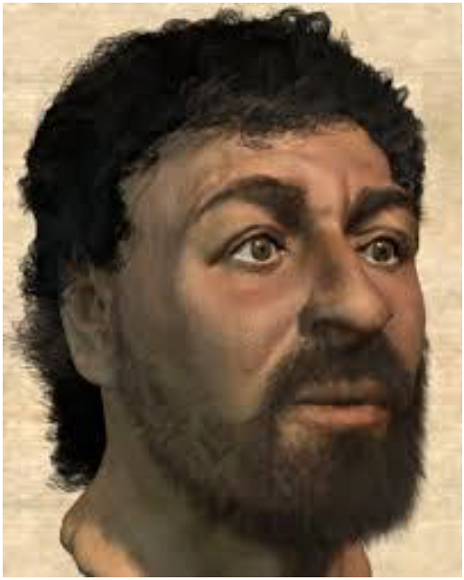
\includegraphics[scale=0.5]{graphics/jesus.PNG}
\captionof{figure}{Wie er vermutlich Aussah}
\end{minipage}
\begin{minipage}[t]{0.49\textwidth}
\centering
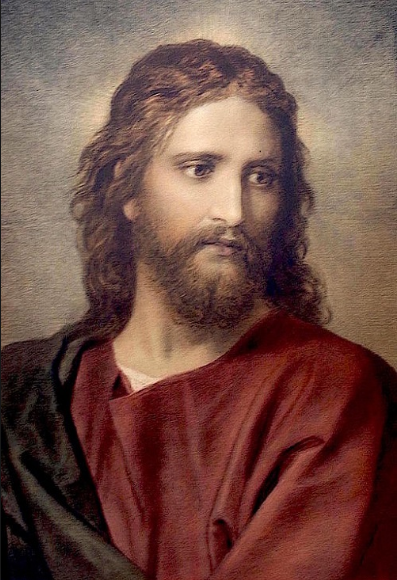
\includegraphics[scale=0.5]{graphics/jesus_c.PNG}
\captionof{figure}{Wie er in Büchern und Bildern aussieht}
\end{minipage}